\documentclass[12pt]{article}

\usepackage[margin = .8in]{geometry}
\usepackage{amsmath}
\usepackage{graphicx}
\usepackage{multicol}

\usepackage{fancyhdr}
\pagestyle{fancy}

\lhead{Math F113X: Math and Society}
\rhead{Graph Theory}

\usepackage{tikz}
\usetikzlibrary{calc,trees,positioning,arrows,fit,shapes,calc}

\usepackage{longtable}
\usepackage{tabularx}

\newcommand{\ds}{\displaystyle}
\newcommand{\ans}[1][1in]{\rule{#1}{.5pt}}
\renewcommand{\emph}[1]{\textsf{\textbf{#1}}}

\usepackage{array}
\newcolumntype{L}[1]{>{\raggedright\let\newline\\\arraybackslash\hspace{0pt}}m{#1}}
\newcolumntype{C}[1]{>{\centering\let\newline\\\arraybackslash\hspace{0pt}}m{#1}}
\newcolumntype{R}[1]{>{\raggedleft\let\newline\\\arraybackslash\hspace{0pt}}m{#1}}
\newcommand{\red}[1]{\textcolor{red}{#1}}


\begin{document}


\begin{center}
{\Large  Worksheet:  Modeling with Graphs	}
\end{center}


\noindent \textbf{Group Names:} \hrulefill 

\begin{enumerate}

%========================================================
\item  Six students are in a study group. The table says who has already worked together.

\begin{center}
\begin{tabular}{l|l}
student & has worked with \\ \hline
Ana & Ben, Cleo, Dev \\
Ben & Ana, Cleo \\
Cleo & Ana, Ben, Dev \\
Dev & Ana, Cleo, Eli \\
Eli & Dev \\
Fern & --- \\
\end{tabular}
\end{center}

\begin{enumerate}
\item Draw a graph that represents the situation.

\vspace{2in}

%\begin{center}
%\begin{tikzpicture}[vtx/.style={draw, circle, inner sep = 2 pt}]
%\node[vtx] (A) at (0,0) {Ana};
%\node[vtx] (B) at (2.6,0) {Ben};
%\node[vtx] (C) at (5.2,0) {Cleo};
%\node[vtx] (D) at (0,-2) {Dev};
%\node[vtx] (E) at (2.6,-2) {Eli};
%\node[vtx] (F) at (5.2,-2) {Fern};
%\end{tikzpicture}
%\end{center}

\item What are the vertices in your model? \ans[3.2in]

\item What are the edges? \ans[3.2in]

\item Is your graph connected? \ans[.7in] \ What does that mean \emph{about the study group}?

\vspace{.6in}

\end{enumerate}

%\newpage

%========================================================
\item Below are two graphs. Two graphs are ``the same'' if they have the same edges (regardless of the vertex labels or how they are drawn), and they are different if there is a feature that one has that the other does not.%Are they the same graph? Why or why not?

\begin{center}
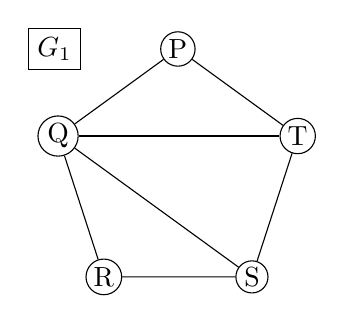
\begin{tikzpicture}[vtx/.style={draw, circle, inner sep = 1 pt}]
\node[vtx] (P) at (90:1.6) {P};
\node[vtx] (Q) at (162:1.6) {Q};
\node[vtx] (R) at (234:1.6) {R};
\node[vtx] (S) at (306:1.6) {S};
\node[vtx] (T) at (18:1.6) {T};
\draw (P) -- (Q) -- (R) -- (S) -- (T) -- (P);
\draw (Q) -- (S);
\draw (Q) -- (T);
\node[draw, left=of P] {$G_{1}$};
\end{tikzpicture}
\hspace{1.1in}
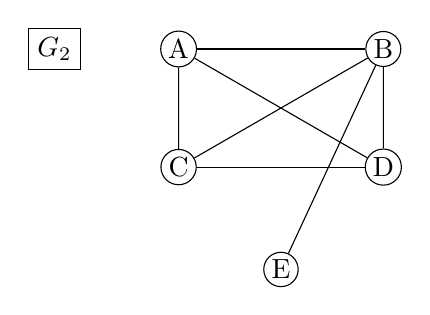
\begin{tikzpicture}[vtx/.style={draw, circle, inner sep = 1 pt}]
\node[vtx] (Q) at (0,0) {A};
\node[vtx] (S) at (2.6,0) {B};
\node[vtx] (P) at (0,-1.5) {C};
\node[vtx] (R) at (2.6,-1.5) {D};
\node[vtx] (T) at (1.3,-2.8) {E};
\draw (Q) -- (S);
\draw (Q) -- (P) (Q) -- (R);
\draw (S) -- (R) (S) -- (T);
\draw (P) -- (R);
\draw (S)--(P);
\node[draw, left =of Q] {$G_{2}$};
\end{tikzpicture}
\end{center}

Same graph? \ans[.7in] Why or why not? (explain)

\vspace{.3in}

\newpage
%========================================================
\item We want to model the following situations. %What graph could do this?

\begin{enumerate}
\item A snowplow must clear every street in a neighborhood.

\emph{vertices:} \ans[1.4in] \quad \emph{edges:} \ans[1.4in]

%\vspace{.2in}

\item A delivery driver must stop at several businesses, once each.

\emph{vertices:} \ans[1.4in] \quad \emph{edges:} \ans[1.4in]

%\vspace{.2in}

\item A utility wants to run fiber to every village in a region as cheaply as possible.

\emph{vertices:} \ans[1.4in] \quad \emph{edges:} \ans[1.4in]

%\vspace{.2in}

%\item Match each of (a), (b), (c) to one of the three questions from the lecture notes.
%
%\smallskip
%
%covers every \emph{edge}: \ans[.5in] \quad visits every \emph{vertex}: \ans[.5in] \quad connects everything as cheaply as possible: \ans[.5in]

\end{enumerate}

%\vfill

%\newpage

%========================================================
\item \emph{Degree.} Graph \emph{W} is shown below, twice.

\begin{center}
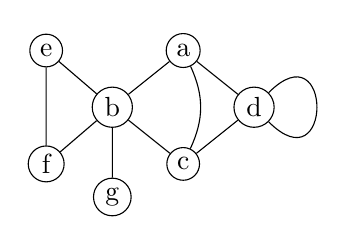
\begin{tikzpicture}[vtx/.style={draw, circle, inner sep = 2 pt}, scale = .6]
\node[vtx] (a) at (0,0) {a};
\node[vtx] (b) at (-1.5,-1.2) {b};
\node[vtx] (c) at (0,-2.4) {c};
\node[vtx] (d) at (1.5,-1.2) {d};
\node[vtx] (e) at (-2.9,0) {e};
\node[vtx] (f) at (-2.9,-2.4) {f};
\node[vtx] (g) at (-1.5,-3.1) {g};
\draw (a) -- (b) -- (c) -- (d) -- (a);
\draw (a) to[bend left = 25] (c);
\draw (d) to[out = -45, in = 45, looseness = 8] (d);
\draw (b) -- (e);
\draw (b) -- (f);
\draw (e) -- (f);
\draw (b) -- (g);
\end{tikzpicture}
\hspace{.9in}
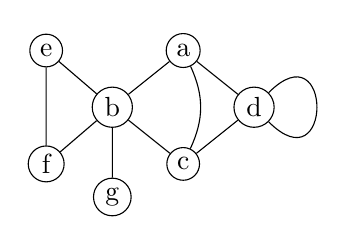
\begin{tikzpicture}[vtx/.style={draw, circle, inner sep = 2 pt}, scale = .6]
\node[vtx] (a) at (0,0) {a};
\node[vtx] (b) at (-1.5,-1.2) {b};
\node[vtx] (c) at (0,-2.4) {c};
\node[vtx] (d) at (1.5,-1.2) {d};
\node[vtx] (e) at (-2.9,0) {e};
\node[vtx] (f) at (-2.9,-2.4) {f};
\node[vtx] (g) at (-1.5,-3.1) {g};
\draw (a) -- (b) -- (c) -- (d) -- (a);
\draw (a) to[bend left = 25] (c);
\draw (d) to[out = -45, in = 45, looseness = 8] (d);
\draw (b) -- (e);
\draw (b) -- (f);
\draw (e) -- (f);
\draw (b) -- (g);
\end{tikzpicture}
\end{center}

\begin{enumerate}
\item Label each vertex of the \emph{right-hand} copy with its degree. Remember a loop counts twice.
\item Which vertex has the largest degree? \ans[.8in]
\item How many edges does \emph{W} have? \ans[.8in]
\item Find a circuit and highlight/draw it on the left-hand graph. \ans
\item Find a path from $e$ to $d$. Write the sequence of vertices \ans[1in]
\item Is there a vertex you could delete that would leave the graph \emph{not} connected? \ans[1cm] Why?


\end{enumerate}

\vspace{.3in}

%========================================================
\item Fill in the table using the graphs on this worksheet.

\begin{center}
{\renewcommand{\arraystretch}{1.6}
\begin{tabular}{c | c | c}
graph & sum of all the degrees & number of edges \\ \hline
study group (\#1) &  & \\ \hline
graph $G_{1}$ in \#2 & & \\ \hline
graph \emph{W} &  & \\ \hline
\end{tabular}
}
\end{center}



\emph{Find a pattern:} the sum of all the degrees of the vertices of a graph is always \ans[1.2in] the number of edges.

\bigskip

Why should that be true? %Think about what each edge contributes to the total.

%\vspace{1in}
%
%%========================================================
%\item \emph{Your turn.} Here is a graph with no context attached.
%
%\begin{center}
%\begin{tikzpicture}[vtx/.style={draw, circle, inner sep = 2 pt}]
%\node[vtx] (1) at (0,0) {};
%\node[vtx] (2) at (1.8,.6) {};
%\node[vtx] (3) at (3.6,0) {};
%\node[vtx] (4) at (1.8,-1.4) {};
%\node[vtx] (5) at (5.2,-1.0) {};
%\draw (1) -- (2) -- (3) -- (4) -- (1);
%\draw (2) -- (4);
%\draw (3) -- (5);
%\end{tikzpicture}
%\end{center}
%
%Invent a situation this graph could model. What do the vertices represent? What do the edges represent? What is a question you would actually want to answer about your situation?
%
%\vspace{2in}

\end{enumerate}

\end{document}
